\section{Introduction}

In Part \ref{part:FD} of this thesis, we are considering Bayesian estimation of Volterra series models in the frequency domain. While Chapter \ref{chap:7} revealed that Gaussian process regression (GPR) can be applied to the NOFRF model, the results were limited to the case of a parallel Hammerstein nonlinear system, as this is the case where the NOFRFs become input independent and thus easy to model in a Bayesian sense. In order to make Bayesian frequency domain estimation more broadly applicable, it is necessary to move to the generalized frequency response function (GFRF) model, where each complex-valued GFRF in the series is related to its corresponding time domain kernel through a multidimensional Fourier transform.

The estimation of GFRFs has been extensively studied in the literature. In one case, an interpolation method for the second order term was developed \cite{Nemeth2002}, which requires multiple input realizations to give an overdetermined problem. Other studies utilized excitations with specifically selected harmonics, however such methods become prohibitively complex for high nonlinear orders, and there is a limit to the number of GFRF elements which can be estimated~\cite{Boyd1983}, \cite{Evans1996}. Alternatively, full GFRF estimates can be obtained from arbitrary excitation by first identifying the time domain Volterra kernels and then transforming to the frequency domain \cite{Vlaar2018}. In the case where a limited frequency band is of interest, then identification directly in the frequency domain is more beneficial with respect to the number of estimated parameters.

The contribution of this chapter is to develop a frequency domain GFRF identification method using GPR, and thus further expand the capabilities of nonparametric Bayesian estimation. As in previous chapters, concepts from \cite{Birpoutsoukis2017} and \cite{Lataire2016} will serve as inspiration in developing the method. In particular, the real/complex Gaussian framework described in Chapter \ref{sec:RCN} is utilized again, and the GFRFs are modeled using prior covariances translated from the time domain functions designed in \cite{Birpoutsoukis2017}.

The proposed approach can obtain GFRF estimates up to an arbitrary nonlinear order using a single multisine input excitation, even though the estimation problem is severely rank deficient. For cases where only a limited frequency band is of interest, the proposed method presents a clear advantage over indirect time domain GPR, which is a property that was also observed for the linear case in \cite{Lataire2016}.

\section{Problem formulation}
\label{sec:ProblemFormulation_GFRFs}

For convenience, the relevant time domain and frequency domain Volterra models will be recalled here for reference throughout the chapter. The original time domain series is given by
\begin{equation}
\begin{split}
y^0(t) &= h_0 + \sum_{m=1}^M y_m(t), \\
y_m(t) &= \sum_{\tau_1 = 0}^{n_m-1} \hdots \sum_{\tau_m=0}^{n_m-1} h_m(\tau_1, \hdots, \tau_m) \prod_{\tau=\tau_1}^{\tau_m} u(t-\tau).
\end{split}
\label{eq:VolterraTimeDomainOutput_GFRFs}
\end{equation}
The GFRF model then relates the (steady-state) input and output spectrum in the frequency domain, i.e.
\begin{equation}
\begin{split}
Y^0(k) &= H_0(k) + \sum_{m=1}^{M} Y_m(k),  \\
Y_m(k) &= \frac{1}{N^{m-1}} \sum_{k_1 + \hdots + k_m = k} H_m(k_1, \hdots,k_m) \prod_{i=1}^{m} U(k_i), 
\end{split}
\label{eqn:GFRFoutputeqn_GFRFs}
\end{equation}
where the GFRFs, $H_m$, are obtained via multidimensional Fourier transforms on the corresponding Volterra kernels, $h_m$, using
\begin{equation}
\label{eqn:GFRF_Transform_GFRFs}
H_m(k_1, \hdots,k_m) = \sum_{\tau_1=0}^{n_m - 1} \hdots \sum_{\tau_m=0}^{n_m-1} h_m(\tau_1,\hdots,\tau_m) e^{\frac{-j2 \pi k_1 \tau_1}{N}} \cdots e^{\frac{-j2 \pi k_m \tau_m}{N}}.
\end{equation}

The nonlinear system identification problem is now formulated in the frequency domain under steady-state conditions, using the following assumptions and notation: 
\begin{assum}
\label{assum:white_noise_Volterra_output}
The measured output, $\{y(t)\}_{t=0}^{N-1}$, is a Volterra output corrupted by white noise, i.e.
\begin{equation}
y(t) = y^0(t) + e(t); \; \; \; \; e(t) \sim \mathcal{N}(0,\sigma^2),
\label{eqn:VolterraWithNoise_transients}
\end{equation}
where $y^0(t)$ is the noise-free Volterra output from (\ref{eq:VolterraTimeDomainOutput_GFRFs}).
\end{assum}
\begin{assum}[Steady-state]
The measured input $\{u(t)\}_{t=0}^{N-1}$ is one period of an N-periodic sequence which has been applied to the system for a sufficiently long time  such that the system is in steady-state with a corresponding N-periodic output response, $\{y^0(t)\}_{t=0}^{N-1}$, whose spectrum can be given by the steady-state GFRF model (\ref{eqn:GFRFoutputeqn_GFRFs}).
\label{assum:steadystate_transients}
\end{assum}
%\begin{assum}[Alias-free]
%\label{assum:antialias_input}
%The input DFT spectrum for non-negative frequencies, $\{U(k): k \in \mathbb{Z}, 0 \leq k \leq N/2\}$, has non-zero values only in the set of indices $\mathbf{k_u} \subset \{0,\hdots,\floor*{\frac{N}{2M}} \}$, where $\floor*{\cdot}$ is the floor operator.
%\end{assum}
\begin{notation}
The set of DFT indices, $k$, for which the input spectrum, $\{U(k): k \in \mathbb{Z}, 0 \leq k \leq N/2\}$, is non-zero is denoted by $\mathbf{k_u}$. Likewise, the set of indices for which the output spectrum, $\{Y(k): k \in \mathbb{Z}, 0 \leq k \leq N/2\}$, is non-zero (due to input excitation) is denoted by $\mathbf{k_y}$ (see \cite{Lang1997} for the precise definition of this set for a given $U(k)$ and $M$).
\end{notation}
\begin{notation}
The frequencies of interest for estimation are given by the set \begin{equation} \mathbf{k_e} = -\mathbf{k_u} \cup \mathbf{k_u}. \end{equation}
\end{notation}
Given Assumptions \ref{assum:white_noise_Volterra_output} and \ref{assum:steadystate_transients}, the goal is to estimate the GFRF elements, $H_0$ and $H_m(k_1, \hdots,k_m)$ $\forall k_1, \hdots,k_m \in \mathbf{k_e}$ and $m = 1,\hdots,M$.

\section{Gaussian process regression for GFRFs}
\label{sec:GPR_GFRFs}

Given the assumptions and problem formulation described in Section \ref{sec:ProblemFormulation_GFRFs}, a GPR method is developed in this section. The hybrid real/complex normal distribution will be required for this purpose, since every GFRF contains both complex \emph{and} strictly real components. Thus, the notation and properties introduced in Chapter \ref{sec:RCN} will also be used in this chapter.

\subsection{GFRFs as real/complex Gaussian vectors}

Any set of GFRF parameters can be arranged into a real/complex vector, as outlined in the following definition.

\begin{defn}
The $m$-dimensional array containing $H_m(k_1, \hdots,k_m), \ \forall k_1, \hdots,k_m \in \mathbf{k_e}$ has a real/complex vectorized form (shown in (\ref{eqn:RCG_vector_defn})) which will be denoted by 
\begin{equation}
\label{eqn:GFRF_RCG_vector}
H_m^{\mathcal{V}} = \begin{bmatrix} H_m^{\mathbb{R}} \\ H_m^{\mathbb{C}} \end{bmatrix}, 
\end{equation}
where $H_m^{\mathbb{R}}$ contains the strictly real components.
\end{defn}

Unlike in \cite{Lataire2016} and Chapter \ref{chap:7}, where the one-dimensional frequency functions are strictly real only at zero frequency, higher order GFRFs originating from symmetric Volterra kernels present a larger set of real components. Since we are required to express the vectorized GFRFs in the form dictated by (\ref{eqn:GFRF_RCG_vector}), it is important to identify the location of all strictly real elements, as addressed in the following theorem.

\begin{thm}
\label{thm:GFRF_real_elements}
Consider a symmetric $m$\textsuperscript{th} order Volterra kernel, $h_m(\tau_1, \hdots, \tau_m)$, as defined in (\ref{eq:VolterraTimeDomainOutput_GFRFs}), and its corresponding GFRF, $H_m(k_1, \hdots,k_m)$, as defined in (\ref{eqn:GFRF_Transform_GFRFs}). The strictly real components of $H_m$ are defined by the set of DFT indices,
\begin{align*}
\mathbf{k}_m^{\mathbb{R}} = \{k_1, \hdots, k_m \in \mathbb{Z}: \sum_{\mathcal{I} \in S_m(X)} \sin \bigg( \frac{2 \pi}{N} (k_1 \tau_{i_1} + \hdots + k_m \tau_{i_m}) \bigg) = 0 \; \; \forall \tau_i \in \mathbb{N} \}, 
\end{align*}
where $\mathcal{I} = [i_1, \hdots, i_m]$, and $S_m(X)$ denotes the set of all permutations of the vector $X = [1, 2, \hdots,m]$.
\end{thm}
\begin{proof*}
Taking the imaginary part of (\ref{eqn:GFRF_Transform_GFRFs}), we obtain
\begin{align}
\mathfrak{I} \{ &H_m(k_1,\hdots,k_m) \} = \sum_{\tau_1 = 0}^{n_m-1} \hdots \sum_{\tau_m = 0}^{n_m-1} h_m(\tau_1,\hdots,\tau_m) \sin(\frac{2 \pi}{N}(k_1 \tau_1 + \hdots + k_m \tau_m)).
\end{align}
For a symmetric kernel $h_m$, the Fourier transformation will be independent of the ordering of the lags, $\tau_1,\hdots,\tau_m$, so it is equivalent to take an average over all lag permutations,
\begin{align}
\mathfrak{I} \{ &H_m(k_1,\hdots,k_m) \} \nonumber \\
&= \frac{1}{m!} \sum_{\mathcal{I} \in S_m(X)} \Bigg[ \sum_{\tau_1 = 0}^{n_m-1} \hdots \sum_{\tau_m = 0}^{n_m-1} h_m(\tau_{i_1},\hdots,\tau_{i_m}) \sin \bigg( \frac{2 \pi}{N}(k_1 \tau_{i_1} + \hdots + k_m \tau_{i_m}) \bigg) \Bigg] \\
&= \frac{1}{m!} \sum_{\tau_1 = 0}^{n_m-1} \hdots \sum_{\tau_m = 0}^{n_m-1} h_m(\tau_{1},\hdots,\tau_{m}) \sum_{\mathcal{I} \in S_m(X)} \sin \bigg( \frac{2 \pi}{N}(k_1 \tau_{i_1} + \hdots + k_m \tau_{i_m}) \bigg).
\end{align}
Thus, for an arbitrary symmetric $h_m$, strictly real elements of $H_m$ are guaranteed only when
\begin{align*}
\sum_{\mathcal{I} \in S_m(X)} \sin(\frac{2 \pi}{N}(k_1 \tau_{i_1} + \hdots + k_m \tau_{i_m})) = 0 \; \; \forall \tau_i \in \mathbb{N} 
\end{align*} 
as required. \hfill $\qed$
\end{proof*}

To explicitly locate the strictly real elements within the estimation set, $\mathbf{k_e}$, the result in Theorem \ref{thm:GFRF_real_elements} can be elaborated using the antisymmetry of $\sin()$, as shown below for the first three nonlinear orders. %(i.e. the orders considered in the simulation examples).
\begin{align}
\mathbf{k}_1^{\mathbb{R}} = &\{k_1 \in \mathbf{k_e}: k_1 = 0 \}, \\
\mathbf{k}_2^{\mathbb{R}} = &\{k_1, k_2 \in \mathbf{k_e}: k_1 = -k_2 \}. \\
\mathbf{k}_3^{\mathbb{R}} = &\{k_1,k_2,k_3 \in \mathbf{k_e}: k_1 = -k_2, k_3 = 0 \} \cup \nonumber \\
& \hspace{10mm} \{k_1,k_2,k_3  \in \mathbf{k_e}: k_1 = -k_3, k_2 = 0 \} \cup \nonumber \\
& \hspace{20mm} \{k_1,k_2,k_3  \in \mathbf{k_e}: k_2 = -k_3, k_1 = 0 \}. 
\end{align}
Note that the set for the first order GFRF, $\mathbf{k}_1^{\mathbb{R}}$, can only contain the zero frequency entry, as is the case for a linear FRF. The multidimensional GFRFs, however, possess larger sets in general.

\subsection{The Gaussian assumption}

The following Gaussian assumptions are placed on the vectorized GFRF quantities, $H_m^{\mathcal{V}}$.  
\begin{assum}
\label{GFRF_GaussianAssumption}
$H_m^{\mathcal{V}}$ is real/complex normally distributed with zero mean and augmented covariance $\Sigma_m$, i.e.
\begin{equation} 
\label{GFRF_GaussianDefn}
H_m^{\mathcal{V}} \sim \mathcal{RCN}(0,\Sigma_m) ,
\end{equation}
where $\Sigma_m$ is constructed from the covariance and relation functions $R_m$, $Q_m$, $K_m$ and $C_m$ as in (\ref{eqn:augmented_covariance}).
\end{assum}
\begin{assum}
\label{GFRF_IndependenceAssumption}
Two (real/complex vectorized) Gaussian GFRFs of different orders are independent, i.e. $H_i^{\mathcal{V}}$ and $H_j^{\mathcal{V}}$ are independent for $i \neq j$.
\end{assum}
The assumptions \ref{GFRF_GaussianAssumption} and \ref{GFRF_IndependenceAssumption} are consistent with those made in \cite{Birpoutsoukis2017} and \cite{Lataire2016}, as well as in previous chapters of this thesis. They will be used in the sequel to derive the output spectrum distribution and define the GPR procedure for GFRF estimation.

\subsection{Prior covariance design}

For multidimensional Volterra kernels, prior covariance functions have already been constructed in the time domain \cite{Birpoutsoukis2017}, \cite{Birpoutsoukis2017c}, by applying a TC or DC structure along multiple perpendicular regularizing directions. The same approach was adopted for the time domain methods in this thesis, in Chapters 4, 5 and 6. The resulting covariance matrices are guaranteed to be valid and produce stable kernel realizations.

In order to construct a frequency domain analog to the Volterra kernel covariance function, we note that there exists a linear transformation between the vectorized kernel $h_m^{\mathcal{V}}$ and its frequency domain counterpart, $H_m^{\mathcal{V}}$, which will be denoted $F_m$, i.e.
\begin{equation}
H_m^{\mathcal{V}} = \begin{bmatrix} H_m^{\mathbb{R}} \\ H_m^{\mathbb{C}} \end{bmatrix} = \begin{bmatrix} F_m^{\mathbb{R}} \\ F_m^{\mathbb{C}} \end{bmatrix} h_m^{\mathcal{V}} = F_m h_m^{\mathcal{V}},
\end{equation}
where $F_m^{\mathbb{R}}$ produces $H_m^{\mathbb{R}}$ and $F_m^{\mathbb{C}}$ produces $H_m^{\mathbb{C}}$. While it is clear from (\ref{eqn:GFRF_Transform_GFRFs}) that $F_m$ should contain appropriate products of exponentials, a more rigorous approach for obtaining the explicit form of $F_m$ and its submatrices requires the following theorem.

\begin{thm}
\label{thm:ND-DFTs}
Consider the m-dimensional array $w_m \in \mathbb{R}^{N \times \hdots \times N}$, and its m-dimensional DFT, $W_m \in \mathbb{C}^{N \times \hdots \times N}$. Consider also their vectorized forms, $w_m^{\mathcal{V}}\in \mathbb{R}^{N^{m}}$ and $W_m^{\mathcal{V}} \in \mathbb{C}^{N^{m}}$, where vectorization is performed such that 
\begin{align*}
w_m^{\mathcal{V}} = \big[ w_m(1,1,\hdots,1), &w_m(2,1,\hdots,1),\hdots, \\
& \; \; w_m(N,1,\hdots,1), w_m(1,2,\hdots,1), \hdots, w_m(N,N,\hdots,N) \big],
\end{align*}
and likewise for $W_m^{\mathcal{V}}$. The vectorized arrays are related by,
\begin{equation}
W_m^{\mathcal{V}} = \Psi_m w_m^{\mathcal{V}},
\end{equation}
where $\Psi_m$ can be obtained from the recursive definition,
\begin{align}
\Psi_p = \Psi_{p-1} \otimes \Psi_1,  \; \; p = 2, 3, \hdots, m  
\end{align}
and where $\Psi_1$ is the $N \times N$ DFT matrix.
\end{thm}

\begin{proof*}
For $m=1$, by definition we have:
\begin{equation}
W_1^{\mathcal{V}} = \Psi_1 w_1^{\mathcal{V}}
\end{equation}
For $m=2$, the DFT is applied in each dimension separately:
\begin{align}
W_2 &= \Psi_1 w_2 \Psi_1^T \\
&= \underbrace{[\Psi_1 \otimes \Psi_1]}_{\Psi_2} w_2^{\mathcal{V}},
\end{align}
by the well known property of Kronecker products. 

For tensor $W_m = \{ W_{i_1,\hdots,i_m} \}_{i_1,\hdots,i_m = 0}^{N-1}$, let the $m-1$ dimension tensor $W_m^{(k)}$ be given by $\{ W_{i_1,\hdots,i_{m-1},k} \}_{i_1,\hdots,i_{m-1} = 0}^{N-1}$. 

Assuming $W_{p-1}^{\mathcal{V}} = \Psi_{p-1} w_{p-1}^{\mathcal{V}}$, then by induction:
\begin{align}
\big[ {W_{p}^{(1)}}^{\mathcal{V}} \; \hdots \; {W_{p}^{(N)}}^{\mathcal{V}} \big]  &= \big[ \Psi_{p-1} {w_{p}^{(1)}}^{\mathcal{V}} \; \hdots \; \Psi_{p-1} {w_{p}^{(N)}}^{\mathcal{V}} \big] \Psi_1^T \\
&= \Psi_{p-1} \big[ {w_{p}^{(1)}}^{\mathcal{V}} \; \hdots \; {w_{p}^{(N)}}^{\mathcal{V}} \big] \Psi_1^T \\
\implies W_{p}^{\mathcal{V}} &= \underbrace{[\Psi_{p-1} \otimes \Psi_1]}_{\Psi_{p}} w_{p}^{\mathcal{V}}
\end{align}
again using the Kronecker product property. Thus, $\Psi_{p} = \Psi_{p-1} \otimes \Psi_1 $ as required \hfill  $\qed$

\end{proof*} 

Assuming $h_m^{\mathcal{V}}$ is vectorized as described in Theorem \ref{thm:ND-DFTs}, we can form $F_m$ by first computing the matrix $\Psi_m$, then rearranging and removing rows to correspond to a desired vectorization of $H_m^{\mathcal{V}}$ which satisfies the required form in (\ref{eqn:GFRF_RCG_vector}).

The transformation can now be used to convert time domain covariance functions to the frequency domain,
\begin{equation}
\begin{split}
R_m &= \textbf{E} \{ H_m^{\mathbb{R}} {H_m^{\mathbb{R}}}^T\} = F_m^{\mathbb{R}} \textbf{E} \{ h_m^{\mathcal{V}} {h_m^{\mathcal{V}}}^T \} {F_m^{\mathbb{R}}}^T = F_m^{\mathbb{R}} P_m {F_m^{\mathbb{R}}}^T \\
Q_m &= \textbf{E} \{ H_m^{\mathbb{R}} {H_m^{\mathbb{C}}}^H\} = F_m^{\mathbb{R}} \textbf{E} \{ h_m^{\mathcal{V}} {h_m^{\mathcal{V}}}^T \} {F_m^{\mathbb{C}}}^H = F_m^{\mathbb{R}} P_m {F_m^{\mathbb{C}}}^H \\
K_m &= \textbf{E} \{ H_m^{\mathbb{C}} {H_m^{\mathbb{C}}}^H\} = F_m^{\mathbb{C}} \textbf{E} \{ h_m^{\mathcal{V}} {h_m^{\mathcal{V}}}^T \} {F_m^{\mathbb{C}}}^H = F_m^{\mathbb{C}} P_m {F_m^{\mathbb{C}}}^H \\
C_m &= \textbf{E} \{ H_m^{\mathbb{C}}{H_m^{\mathbb{C}}}^T\} = F_m^{\mathbb{C}} \textbf{E} \{ h_m^{\mathcal{V}} {h_m^{\mathcal{V}}}^T \} {F_m^{\mathbb{C}}}^T = F_m^{\mathbb{C}} P_m {F_m^{\mathbb{C}}}^T 
\end{split}
\label{eq:CovarianceRelationTransforms_GFRFs}
\end{equation}
where $P_m =  \textbf{E} \{ h_m^{\mathcal{V}} {h_m^{\mathcal{V}}}^T \}$ denotes the tunable TC/DC-based covariance structure designed in~\cite{Birpoutsoukis2017} and discussed in Chapter \ref{sec:RegVolterraTD} of this thesis.

The full augmented covariance, $\Sigma_m$, for the $m$\textsuperscript{th} GFRF is constructed as in (\ref{eqn:augmented_covariance}), i.e.
\begin{equation}
\Sigma_m = \begin{bmatrix}  R_m & Q_m & \overline{Q_m} \\ {Q_m}^H & K_m & C_m \\ \overline{{Q_m}^H} & {C_m}^H & \overline{K_m}\end{bmatrix}. \label{eqn:augmented_covariance_GFRFs}
\end{equation} 

\begin{rem}
In practice, symmetry must be enforced in both the time and frequency domain kernels to guarantee a unique Volterra series representation \cite{Schetzen1980}. Thus, we are required to modify the transformation matrices, $F_m$, by removing the columns which correspond to redundant time domain parameters, and removing rows that correspond to redundant frequency domain parameters. As an example, see Figure \ref{fig:BandLimitedVisual} in Section \ref{sec:FDvsTD_GFRFs} for the symmetry axes of a second order kernel and GFRF, which are used to dictate the location of unique and redundant parameters in those series terms.  
\end{rem}

\subsection{Deriving the MAP estimate}

First we must derive the output spectrum distribution for $Y(\mathbf{k_y})$, which requires the restructuring of the model equation (\ref{eqn:GFRFoutputeqn_GFRFs}) into the regression form,
\begin{align}
Y(\mathbf{k_y}) &=  [\Phi_1 \hdots \Phi_M] [{H_1^{\mathcal{V}}}^T \hdots {H_M^{\mathcal{V}}}^T]^T + E(\mathbf{k_y}) \nonumber \\
&= \Phi H + E,
\label{eqn:GFRF_OutputSpectrum}
\end{align}
where $E$ is the (assumed) i.i.d. error vector in the frequency domain, and $\Phi_m$ is an appropriate regressor containing the input spectrum products corresponding to $H_m^{\mathcal{V}}$. Note that symmetry should also be enforced in the GFRFs here, which should be reflected in the design of the regressors. 

Now $Y(\mathbf{k_y})$, being formed from the DFT of the real signal $y(t)$, will also be a real/complex vector in the case where $0 \in \mathbf{k_y}$. Thus, we extend (\ref{eqn:GFRF_OutputSpectrum}) to the augmented output case, resulting in
\begin{align}
\label{AugmentedModel}
\widetilde{Y}(\mathbf{k_y}) &=  [\widetilde{\Phi_1} \hdots \widetilde{\Phi_M}] [\widetilde{H_1^{\mathcal{V}}}^T \hdots \widetilde{H_M^{\mathcal{V}}}^T]^T + \widetilde{E}(\mathbf{k_y}) \nonumber \\
&= \widetilde{\Phi}\widetilde{H} + \widetilde{E}.
\end{align}
The augmented regressors can be constructed as
\begin{equation}
\widetilde{\Phi_m} = \begin{bmatrix}\Phi_m^{\mathbb{R}} & \Phi_m^{\mathbb{RC}} & 0 & 0 \\0 & 0 & \Phi_m^{\mathbb{C}} & 0 \\ 0 & 0 & 0 & \overline{\Phi_m^{\mathbb{C}}} \end{bmatrix},
\end{equation}
where $\Phi_m^{\mathbb{R}}$ maps the contribution of $H_m^{\mathbb{R}}$ to $Y(0)$, and $\Phi_m^{\mathbb{RC}}$ maps the contribution to $Y(0)$ from complex GFRF components. Note that this formulation dictates (to some extent) the required ordering of the vector $H_m^{\mathcal{V}}$. 

\begin{rem}
\label{rem:GFRF_RankDeficiency}
When $\Phi$ is constructed from a single input/output realization as in (\ref{eqn:GFRF_OutputSpectrum}), the associated linear regression problem will be severely rank deficient for $M>1$. While it is possible to make the problem overdetermined by `stacking' a sufficient number of unique input/output realizations (similarly to Chapter \ref{sec:NOFRF_MultipleRealizations}), we will focus on the rank deficient case in this chapter to highlight the flexibility of GPR.
\end{rem}

From (\ref{AugmentedModel}), the output spectrum distribution is derived as follows.
\begin{thm}
For a system whose output is given by (\ref{eqn:VolterraWithNoise_transients}), with Gaussian $H_m^{\mathcal{V}} \sim \mathcal{RCN}(0,\Sigma_m)$ as described in (\ref{GFRF_GaussianDefn}), the output spectrum $Y(\mathbf{k_y})$ is real/complex normally distributed as follows,
\begin{equation}
\begin{split}
\label{OutputSpectrumThm}
Y(\mathbf{k_y}) &\sim \mathcal{RCN}(0,\Sigma_Y), \\
\text{where } \Sigma_Y &= \widetilde{\Phi}\Sigma_{tot} \widetilde{\Phi}^H + \sigma^2 I \\
\text{and } \Sigma_{tot} &= \begin{bmatrix} \Sigma_1 & &0 \\ & \ddots & \\ 0 & & \Sigma_M \end{bmatrix}.
\end{split}
\end{equation}
\end{thm}

\begin{proof*}
Follows directly from (\ref{AugmentedModel}), Assumptions \ref{assum:white_noise_Volterra_output}, \ref{GFRF_GaussianAssumption} and \ref{GFRF_IndependenceAssumption}, and the properties of real/complex normal distributions. \hfill $\qed$
\end{proof*}

Finally, maximum a posteriori (MAP) estimates for the GFRFs can be obtained from the joint distribution of $Y$ and $H$, by computing the mean of the conditional distribution $H|Y$. The result is provided in the following theorem.

\begin{thm}
The MAP estimate of $\widetilde{H}$ in (\ref{AugmentedModel}) is
\begin{equation}
\label{eqn:GFRF_MAP}
\hat{{\widetilde{H}}}_{MAP} = \Sigma_{tot} \widetilde{\Phi}^H \Sigma_Y^{-1} \widetilde{Y}
\end{equation}
\end{thm}

\begin{proof*}
Follows from the properties of real/complex normal distributions \cite{Lataire2016}. \hfill $\qed$
\end{proof*}

\subsection{Hyperparameter tuning}

We must optimize the hyperparameters, $\eta$, describing each covariance function $P_m(\eta)$, which are in turn used to construct $\Sigma_m$ in (\ref{eq:CovarianceRelationTransforms_GFRFs}). As in \cite{Birpoutsoukis2017} and \cite{Lataire2016}, this chapter will use a marginal likelihood maximization (MLM), i.e.
\begin{equation}
\label{eqn:GFRF_hyperparam_tuning}
\hat{\eta} = \text{arg } \underset{\eta}{\text{min }} \widetilde{Y}(\mathbf{k_y})^H \Sigma_Y^{-1}(\eta) \widetilde{Y}(\mathbf{k_y}) + \text{log det } \Sigma_Y(\eta).
\end{equation}

\begin{rem}
The disadvantages of using a MLM approach were highlighted in Chapter \ref{chap:4} for the time domain case. The same situation exists in the frequency domain for GFRFs, i.e. the dimension of the search space in (\ref{eqn:GFRF_hyperparam_tuning}) grows quadratically with the maximum nonlinear order, $M$, and hence the computational burden for the optimization grows even more rapidly. An equivalent EM approach to that of Algorithm \ref{alg:EMtuning} in Chapter \ref{chap:4} can be derived, in an almost identical fashion, for the GFRF estimation problem. The EM tuning method is recommended when $M$ is large.
\end{rem}

\subsection{Comparison with the indirect time domain approach}
\label{sec:FDvsTD_GFRFs}

There is another viable approach for estimating GFRFs under rank deficient conditions, which is to first compute regularized Volterra kernel estimates in the time domain with memory length $n_m = N$, and subsequently transform them using (\ref{eqn:GFRF_Transform_GFRFs}). One advantage of this indirect approach is the freedom to use input/output measurements of arbitrary length which are not necessarily at steady-state, whereas the method proposed here requires such constraints. 

If we are only interested in GFRF estimation for a \emph{specific frequency band}, then the time domain approach has a severe disadvantage when compared to the frequency domain method proposed here. With an indirect time domain approach, we are required to estimate the full set of kernel parameters regardless of frequency band, since each frequency domain parameter depends on the \emph{entire} time domain set (see (\ref{eqn:GFRF_Transform_GFRFs})). In direct frequency domain estimation, the limited frequency band directly reduces the set of parameters to be estimated, and the magnitude of reduction grows rapidly with increasing GFRF order, $m$, since the band is limited along every dimension of the GFRFs. 

An example of this parameter reduction concept is visualized in Figure \ref{fig:BandLimitedVisual} for a second order example with $N=n_2=21$. We excite a discrete set of frequencies, $\mathbf{k_u} = \{ 3,4,5,6,7 \}$, and compare the number of parameters requiring estimation in each domain. It is clear that limiting the excited frequency band in two dimensions significantly reduces the parameter set for $H_2$ to 55 parameters (5 real, 25 complex), while for $h_2$ the full set of unique Volterra coefficients (231 real) is still required.

\begin{figure}[h]
\centering
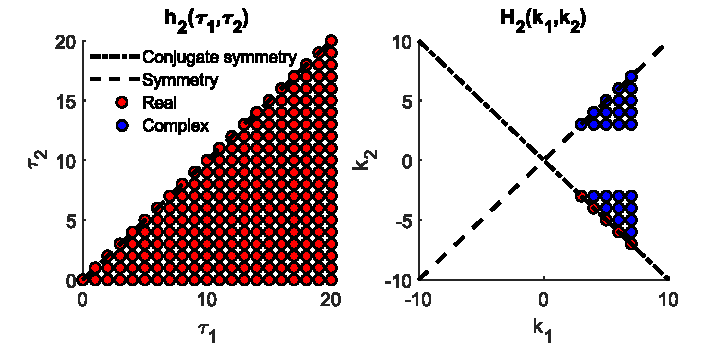
\includegraphics[width = 0.85\textwidth]{Chapter8_GFRFs/LimitedBandParams_paper.pdf}
\caption{Parameters requiring estimation in second order band-limited example where $\mathbf{k_u} = \{ 3,4,5,6,7 \}$, using a time domain approach (left) and using a direct frequency domain approach (right)}
\label{fig:BandLimitedVisual}
\end{figure}

\section{Simulation examples}

Two simulation studies are presented here in order to demonstrate the performance of the proposed method. The first study considers GFRF estimation in a noise-free setting, but using only period of a multisine excitation such that the problem is severely rank-deficient. In the second study, measurement noise is included and the frequencies of interest are limited to a narrow band. For this case a Monte Carlo study is used to compare the proposed GPR method against an indirect time domain approach. 

\subsection{Study 1: rank deficient noise-free case}
\label{sec:GFRF_noisefree_ex}

In the first study, Volterra system outputs are generated using the block structures in Figure \ref{fig:GFRF_WienerStructure}, where the left structure (a) is in a parallel Wiener configuration, and the right structure (b) has a parallel Hammerstein configuration. The linear filters in each structure are defined in the $z$-domain as
$$G_1(z) = \frac{3z}{z^2 -1.8z + 0.84}, \; \; \;  G_2(z) = 0.25 G_1(z).$$
The input, $u(t)$, is given by a periodic multisine with period $N = 80$ and $\mathbf{k_u} = \{0, 1, 2, \hdots, 19\}$, which is applied for 10 periods before taking the final period of measurements for estimation purposes, such that all transient effects are essentially negligible. 

\begin{figure}[!h]
\centering
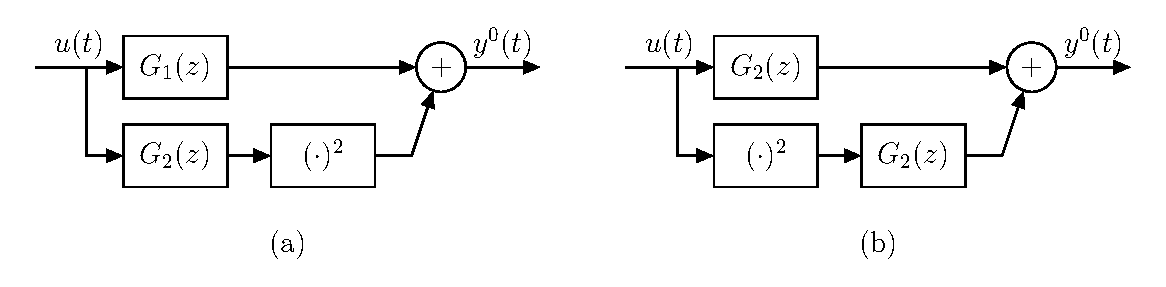
\includegraphics[width = 1\textwidth]{Chapter8_GFRFs/ParallelWienerAndHamm_GFRFs.pdf}
\caption{System structures used for data generation in the rank deficient noise-free case}
\label{fig:GFRF_WienerStructure}
\end{figure}

We consider identification of each system's nonzero GFRFs, $H_1$ and $H_2$, assuming memory lengths $n_1=n_2=N$. The resulting estimation problems are severely rank deficient, with 780 unique parameters requiring estimation, and only 77 corresponding output spectrum measurements. Applying the proposed GPR method, the GFRF estimates are given in Figures \ref{fig:GFRF_Noisefree_estimates} (for structure (a)) and \ref{fig:GFRF_Noisefree_estimates_b} (for structure (b)) alongside the true GFRFs, which can be obtained analytically from the system structure (see Chapter \ref{sec:BlockStructureRelationship}). Despite severe rank deficiency, it is clearly seen that a good result is achieved for each system at both GFRF orders.  

\begin{figure}[!h]
\centering
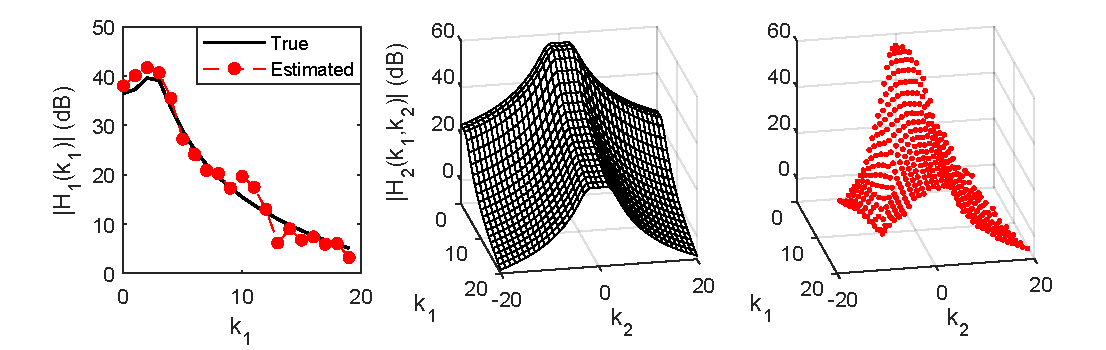
\includegraphics[width = 1.05\textwidth]{Chapter8_GFRFs/WienerExampleEstimates_split2.pdf}
%\caption{First order GFRF estimate (left) and selected slices of the second order GFRF estimate (right)}
\caption{Structure (a) - magnitude plots for the first order GFRF estimate (left), true 2nd order GFRF (middle) and 2nd order estimate for unique parameters (right)}
\label{fig:GFRF_Noisefree_estimates}
\end{figure}

\begin{figure}[!h]
\centering
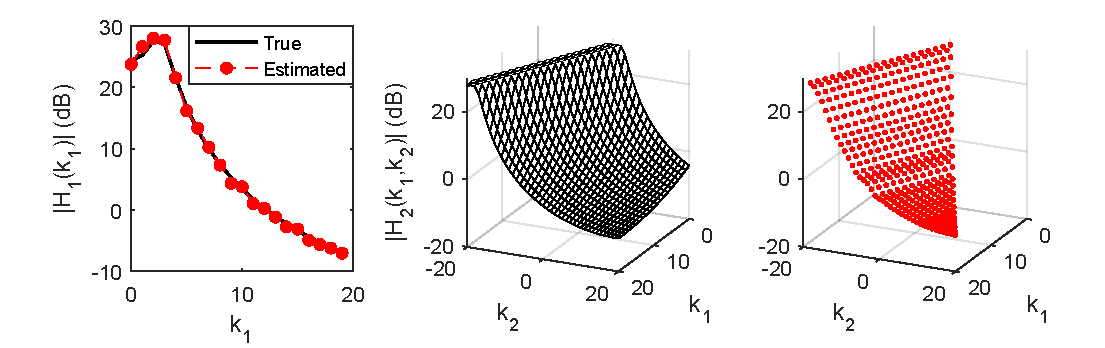
\includegraphics[width = 1.05\textwidth]{Chapter8_GFRFs/HammersteinExampleEstimates_split.pdf}
%\caption{First order GFRF estimate (left) and selected slices of the second order GFRF estimate (right)}
\caption{Structure (b) - magnitude plots for the first order GFRF estimate (left), true 2nd order GFRF (middle) and 2nd order estimate for unique parameters (right)}
\label{fig:GFRF_Noisefree_estimates_b}
\end{figure}

\subsection{Study 2: limited frequency band with measurement noise}

\begin{figure}[!h]
\centering
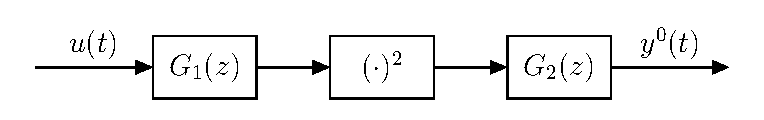
\includegraphics[scale = 0.8]{Chapter8_GFRFs/WienerHamm_GFRFs.pdf}
\caption{Wiener-Hammerstein structure used in the limited frequency band MC study}
\label{fig:GFRF_WienerHammStructure}
\end{figure}

To highlight the advantage of the proposed method over an indirect time domain approach, a Monte Carlo (MC) study is also performed. The noise-free outputs are generated using the Wiener-Hammerstein structure in Figure \ref{fig:GFRF_WienerHammStructure}, with linear filters,
$$G_1(z) = \frac{z-1}{z}, \; \; \;  G_2(z) = \frac{1.07z}{z^2 - 1.72 z + 0.77}.$$
The input is a multisine with period $N=55$ and a limited band of excited frequencies, $\mathbf{k_u} = \{ 4,5,\hdots,12 \}$. The output, $y^0$, is disturbed by additive white measurement noise. Note that the system structure can be represented using a single GFRF, $H_2$, as was discussed in Chapter \ref{sec:BlockStructureRelationship}. We will assume for estimation that $n_2 = N$.   

For the MC study we consider three different noise levels, with each noise level having 100 input/output realizations. For each realization, transient-free estimation data is obtained in the same manner as in Section \ref{sec:GFRF_noisefree_ex}. Estimation of the $H_2$ parameters within the excited band is performed using two separate methods:
\begin{enumerate}
\item \textbf{GPR-FD} - GPR in the frequency domain as developed in this chapter (i.e. using (\ref{eqn:GFRF_MAP}) and (\ref{eqn:GFRF_hyperparam_tuning})), and using the DC structure (\ref{DCext}) for each $P_m$.
\item \textbf{GPR-TD} - GPR in the time domain as presented in \cite{Birpoutsoukis2017} using the DC structure for $P_m$, and using periodicity to define the initial conditions $u(t)$ for $t<0$. GFRF parameters are obtained by the DFT transformation (\ref{eqn:GFRF_Transform_GFRFs}) on each time domain kernel, followed by the elimination of parameters not relevant to the frequency band of interest. 
\end{enumerate}
The noise, $e(t)$, is added in each realization to achieve a Signal-to-Noise Ratio (SNR) of 5, 10 or 20dB.

Estimation errors for each method  and realization are quantified using a normalized mean square error (NMSE) metric, given by 
$$ \textrm{NMSE} = \frac{\frac{1}{n} \sum_{i=1}^{n} | \hat{H}_2^{\mathcal{V}}(i) -  H_2^{\mathcal{V}}(i)|^2}{\frac{1}{n} \sum_{i=1}^{n} |H_2^{\mathcal{V}}(i)|^2},$$
where $n$ is the number of GFRF parameters requiring estimation in the excited frequency band, $\hat{H}_2^{\mathcal{V}}(i)$ is the $i$\textsuperscript{th} element of the GFRF estimate, and $H_2^{\mathcal{V}}(i)$ contains the true GFRF elements in the frequency band of interest.

The errors resulting from each noise level and method are presented as boxplots in Figure \ref{fig:GFRF_MCstudy}. The GPR-FD accuracy is seen to improve with increasing SNR as expected, however it is also clear that for the case of a limited excitation frequency band, the proposed frequency domain regression method performs better than an indirect time domain approach on the same dataset, for the reasons discussed in Section \ref{sec:FDvsTD_GFRFs}. More specifically, the number of unique parameters requiring estimation for GPR-TD is $1540$ (all real), while for GPR-FD it is only $378$ ($14$ real, $182$ complex). 

\begin{figure}[h]
\centering
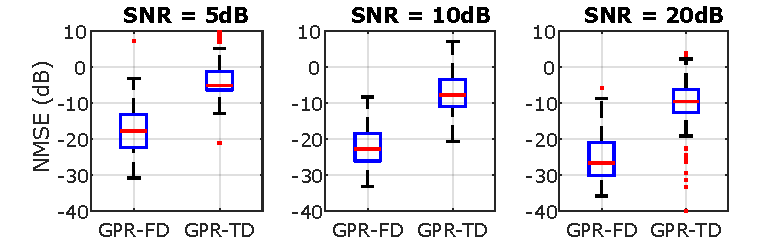
\includegraphics[width = 0.85\textwidth]{Chapter8_GFRFs/GFRF_MCstudy3.pdf}
\caption{NMSEs for the limited frequency band MC study}
\label{fig:GFRF_MCstudy}
\end{figure}

\section{Conclusions}
\label{sec:Conc_GFRFs}

In this chapter, a Gaussian process regression method was presented for the estimation of generalized frequency response functions. The method employs the hybrid real/complex Gaussian framework originally developed for the linear case in \cite{Lataire2016}. The success of the GPR method is dependent on the ability to construct a suitable prior covariance for each GFRF, which is achieved by translating the time domain Volterra kernel covariances designed in \cite{Birpoutsoukis2017}, and hence their properties, to the frequency domain via vectorized Fourier transformations. Numerical examples demonstrated the ability of the method to produce reasonable estimates under severely rank deficient conditions. It was clearly obvious that the proposed method outperforms indirect time domain estimation of GFRFs in the case of a limited frequency band.

When compared to the equivalent linear method in \cite{Lataire2016}, there is an obvious drawback of the method proposed in this thesis, which is the requirement for steady-state conditions during data collection. When the experiment is not performed in steady-state, the measured output will contain an additional transient component with respect to the periodic spectrum predicted by the GFRF model (\ref{eqn:GFRFoutputeqn_GFRFs}). This transient component will negatively affect the estimation accuracy of a method which assumes steady-state whereas the linear case in \cite{Lataire2016} considered the explicit inclusion of a transient function in the model structure. Furthermore, the prior covariance of the transient function (in a Bayesian setting) was shown to be approximately proportional to the FRF covariance under white noise excitation.

The nature of the output transient in a \emph{nonlinear} system is not well understood for the general case, and further investigation is required in order to model both the GFRFs and transient functions in a GPR estimation method. This investigation is performed in Chapter \ref{chap:9}, where the mathematical structure of nonlinear Volterra system transients is derived and examined.